%%%%%%%%%%%%%%%%%%%%%%%%%%%%%%%%%%%%%%%%%%%%%%%%%%%%%%%%%%%%
%% Lecture 03
%%%%%%%%%%%%%%%%%%%%%%%%%%%%%%%%%%%%%%%%%%%%%%%%%%%%%%%%%%%%

\lecture
{03}
{Wednesday, 12 August 2026}
{Introduction to Probability}
{Dr. Nishant Chandgotia}

%%%%%%%%%%%%%%%%%%%%%%%%%%%%%%%%%%%%%%%%%%%%%%%%%%%%%%%%%%%%
\section{Central Limit Theorem and Convergence}

Suppose we toss a fair coin independently $n$ times. The Central Limit
Theorem suggests that

\[
P\!\left(
a<
\frac{\#\text{Heads}-\mu n}
{\sigma\sqrt{n}}
<b
\right)
\longrightarrow
\int_a^b \varphi(x)\,dx,
\qquad
n\to\infty,
\]

where, for a fair coin,
and

\(
\varphi(x)
=
\frac{1}{\sqrt{2\pi}}
e^{-x^2/2}.
\)

%%%%%%%%%%%%%%%%%%%%%%%%%%%%%%%%%%%%%%%%%%%%%%%%%%%%%%%%%%%%

\subsection{Galton Board}

\begin{figure}[H]
    \centering
    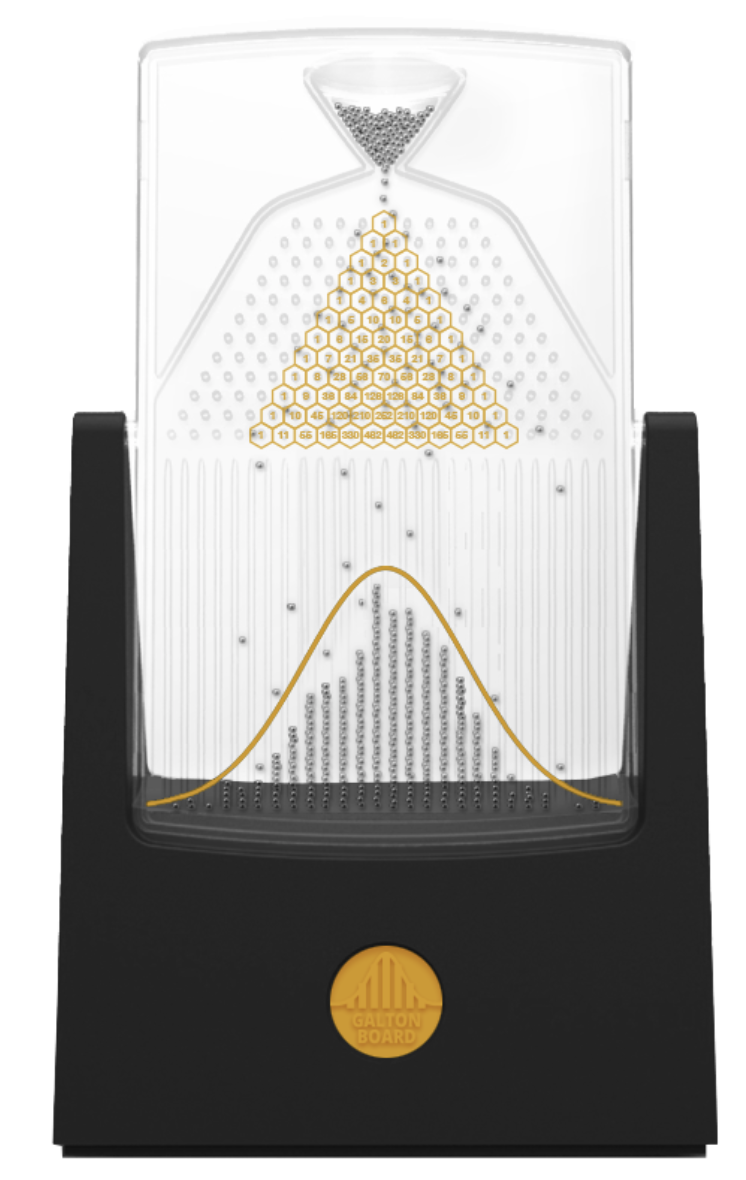
\includegraphics[width=0.3\textwidth]{figures/GaltonBoard.png}
    \caption{Galton board. Source: 
    \href{https://upload.wikimedia.org/wikipedia/commons/d/d2/GaltonBoard.png}
    {Wikimedia Commons}.}
    \label{fig:galton-board}
\end{figure}

The Galton board gives a visual representation of a process whose
distribution approaches a normal distribution.

%%%%%%%%%%%%%%%%%%%%%%%%%%%%%%%%%%%%%%%%%%%%%%%%%%%%%%%%%%%%

\subsection{Random Walk}

A \emph{random walk} is a stochastic process in which the position
changes randomly at each step.

For example, consider a person starting at the origin. At every step,
the person tosses a fair coin:

\[
\begin{cases}
H &\longrightarrow \text{move one step to the right},\\
T &\longrightarrow \text{move one step to the left}.
\end{cases}
\]

This gives the classical one-dimensional symmetric random walk.

There are several natural questions:

\begin{questions}

    \item Will the person return to the origin?

    \item Will the person escape to infinity?

    \item How often will the person return to the origin?

\end{questions}

%%%%%%%%%%%%%%%%%%%%%%%%%%%%%%%%%%%%%%%%%%%%%%%%%%%%%%%%%%%%

\subsection{Convergence in Distribution}

We know, 
\[
\frac{\#\text{Heads}}{n}
\longrightarrow
\frac12.
\]

Now define
\[
f_n
=
\frac{\#\text{Heads}-\mu n}
{\sigma\sqrt{n}}.
\]

Then the Central Limit Theorem states that

\[
P(a<f_n<b)
\longrightarrow
\int_a^b
\frac{1}{\sqrt{2\pi}}
e^{-x^2/2}\,dx.
\]

This leads to the notion of \emph{weak convergence}, or
\emph{convergence in distribution}.

A natural question is whether convergence in distribution implies
almost-sure convergence.

\begin{important}
Convergence in distribution does not, in general, imply almost-sure
convergence.
\end{important}

%%%%%%%%%%%%%%%%%%%%%%%%%%%%%%%%%%%%%%%%%%%%%%%%%%%%%%%%%%%%
\subsection{An Example}

Consider the following random process.

Start with $1$.

Toss a fair coin independently at every step:


\[
\begin{cases}
H &\longrightarrow \text{multiply by }2,\\
T &\longrightarrow \text{multiply by }-2.
\end{cases}
\]

After $n$ steps, define
\[
f_n
=
\frac{\text{product after $n$ steps}}{2^n}.
\]

Since every multiplication contributes either $2$ or $-2$,

\[
f_n\in\{-1,1\}.
\]

Moreover,

\[
P(f_n=1)=\frac12,
\qquad
P(f_n=-1)=\frac12.
\]

Thus the distribution of $f_n$ is the same for every $n$.

However, $f_n$ does not converge almost surely.

\begin{questions}

    \item Does $f_n$ converge almost surely?

    \item Does $f_n$ converge in $L^1$?

    \item Does $f_n$ converge in probability?

\end{questions}

\begin{remark}

The example illustrates that convergence in distribution is a weaker
notion of convergence than almost-sure convergence.

\end{remark}

%%%%%%%%%%%%%%%%%%%%%%%%%%%%%%%%%%%%%%%%%%%%%%%%%%%%%%%%%%%%
\section{Objects in Probability}

There is a close analogy between measure theory and probability theory.

\begin{table}[H]
    \centering
    \caption{Analogy between Measure Theory and Probability}
    \label{tab:measure-probability}

    \renewcommand{\arraystretch}{1.35}

    \begin{tabularx}{\textwidth}{
        >{\raggedright\arraybackslash}X
        >{\raggedright\arraybackslash}X
    }

        \hline

        \textbf{Measure Theory}
        &
        \textbf{Probability}
        \\

        \hline

        Measure space:
        \(\left(\Omega,\mathcal{B},\mu\right)\)
        &
        Probability space:
        \(\left(\Omega,\mathcal{B},\mathbb{P}\right)
        \)

        \\[1ex]

        $\sigma$-algebra $\mathcal{B}$:
        \(A\in\mathcal{B}\), where $\mu(A)$ is defined.
        &
        Event:
        \(A\in\mathcal{B}\), for which
        \(\mathbb{P}(A)\) is defined.

        \\[1ex]

        Elements:
        \(\omega\in\Omega\)
        &
        Outcomes / samples:
        \(\omega\in\Omega\)

        \\[1ex]

        Measurable function:
        \[
        f:(\Omega,\mathcal{B})
        \longrightarrow
        (S,\rho)
        \]
        &
        Random variable:
        \[
        X:(\Omega,\mathcal{B},\mathbb{P})
        \longrightarrow
        (S,\rho)
        \]

        \\[1ex]

        $L^1$-integrability:
        \[
        \int_\Omega |f|\,d\mu<\infty
        \]
        &
        Mean / expectation:
        \[
        \mathbb{E}[X]
        =
        \int_\Omega X\,d\mathbb{P}
        \]

        \\[1ex]

        $L^2$-norm:
        \[
        \|f\|_{L^2}^2
        =
        \int_\Omega |f|^2\,d\mu
        \]
        &
        Variance:
        \[
        \operatorname{Var}(X)
        =
        \mathbb{E}[X^2]
        -
        \mathbb{E}[X]^2
        \]

        \\[1ex]

        Push-forward measure:
        \[
        f_*\mu(A)
        =
        \mu\left(f^{-1}(A)\right)
        \]
        &
        Distribution of $X$:
        \[
        \nu(A)
        =
        \mathbb{P}\left(X^{-1}(A)\right)
        \]

        \\[1ex]

        Fourier transform:
        \[
        \widehat{f}(t)
        =
        \int_{\mathbb{R}}
        e^{itx}f(x)\,dx
        \]
        &
        Characteristic function:
        \[
        \Phi_X(t)
        =
        \mathbb{E}\left[e^{itX}\right]
        \]

        \\[1ex]

        Convergence in measure
        &
        Convergence in probability

        \\[1ex]

        Almost everywhere (a.e.)
        &
        Almost surely (a.s.)

        \\[1ex]

        Convergence in $L^1$
        &
        Convergence in mean.

        \\

        \hline

    \end{tabularx}
\end{table}

%%%%%%%%%%%%%%%%%%%%%%%%%%%%%%%%%%%%%%%%%%%%%%%%%%%%%%%%%%%%

%%%%%%%%%%%%%%%%%%%%%%%%%%%%%%%%%%%%%%%%%%%%%%%%%%%%%%%%%%%%
\section{Sample Space and Sigma Algebra}

The first object in probability is the \emph{sample space}.

\[
\Omega
=
\text{the universe of all possible outcomes}.
\]

For example, for a single coin toss,
\(
\Omega=\{H,T\}.
\)

For a bus arriving at a non-negative time,
\(
\Omega=[0,\infty).
\)

For infinitely many coin tosses,
\(
\Omega=\{H,T\}^{\mathbb{N}}.
\)

An element of this space is an infinite sequence
\(
\omega=(\omega_1,\omega_2,\ldots),
\qquad
\omega_i\in\{H,T\}.
\)

%%%%%%%%%%%%%%%%%%%%%%%%%%%%%%%%%%%%%%%%%%%%%%%%%%%%%%%%%%%%

\subsection{Sigma Algebra}

Let $\mathcal{B}$ denote the $\sigma$-algebra of events.

For a single coin toss,
\(
\mathcal{B}
=
\left\{
\varnothing,
\{H\},
\{T\},
\{H,T\}
\right\}.
\)

For the infinite product space
\(\{H,T\}^{\mathbb{N}}\), the relevant $\sigma$-algebra is generated
by cylinder sets.

%%%%%%%%%%%%%%%%%%%%%%%%%%%%%%%%%%%%%%%%%%%%%%%%%%%%%%%%%%%%

\subsection{Cylinder Sets}

Suppose we are interested only in the first finitely many tosses.

Let
\(
F\subset\mathbb{N}
\)
be a finite set and let
\(
a:F\longrightarrow\{H,T\}
\)
be a fixed assignment of heads and tails.

Define
\(
[a]
=
\left\{
\omega\in\{H,T\}^{\mathbb{N}}
:
\omega_i=a(i)
\text{ for every }i\in F
\right\}.
\)

The set $[a]$ specifies the outcomes of the coordinates belonging to
the finite set $F$, while leaving all other coordinates unrestricted.

Such sets are called \emph{cylinder sets}.

They form a basis for the product topology on
\(
\{H,T\}^{\mathbb{N}}.
\)

We want to be able to assign a probability
\(
\mathbb{P}([a])
\)
to every cylinder set.

For a fair coin, if $|F|=k$, then
\(
\mathbb{P}([a])
=
\frac{1}{2^k}.
\)

%%%%%%%%%%%%%%%%%%%%%%%%%%%%%%%%%%%%%%%%%%%%%%%%%%%%%%%%%%%%



\lectureend
